\subsection{Basical calibration}

\begin{figure}[htbp]
\begin{tabular}{cc}
\begin{minipage}{0.5\hsize}
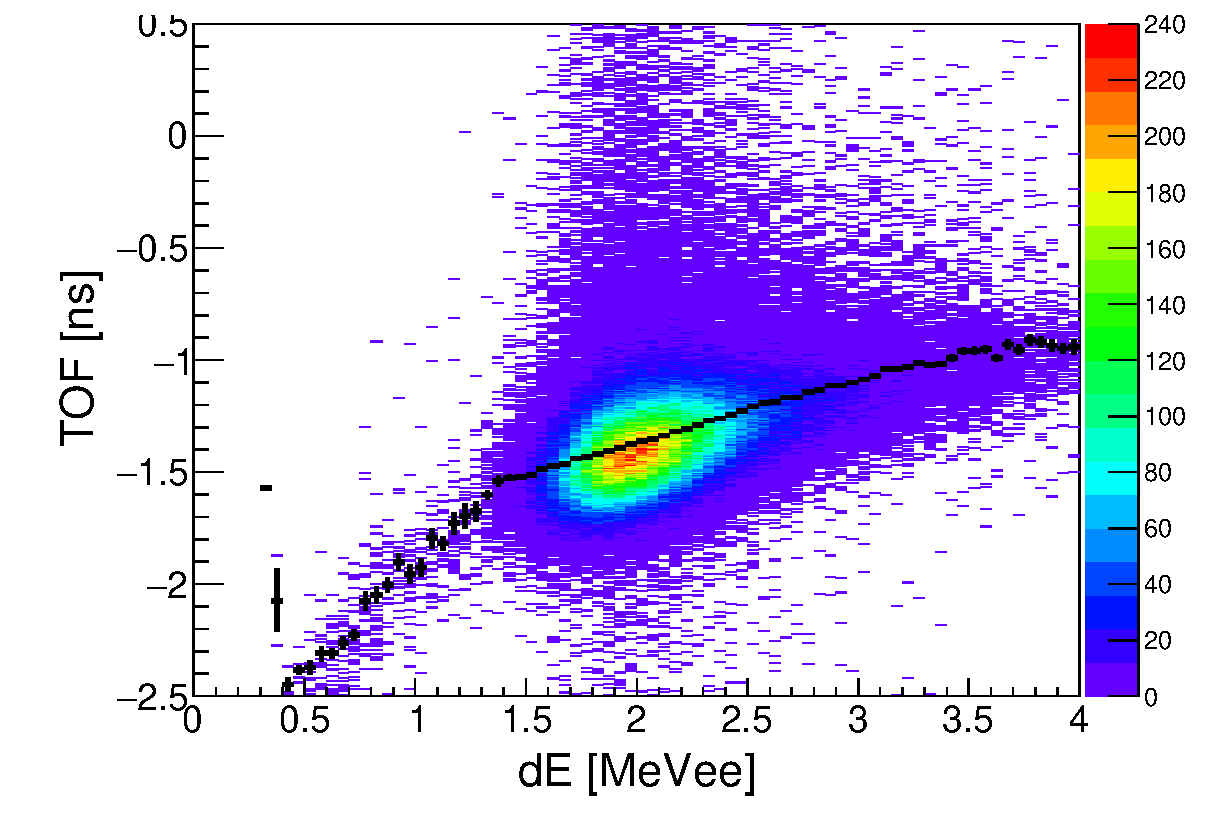
\includegraphics[width=5cm]{../pic/Dron/T0_slew_before.eps}
\end{minipage}
\begin{minipage}{0.5\hsize}
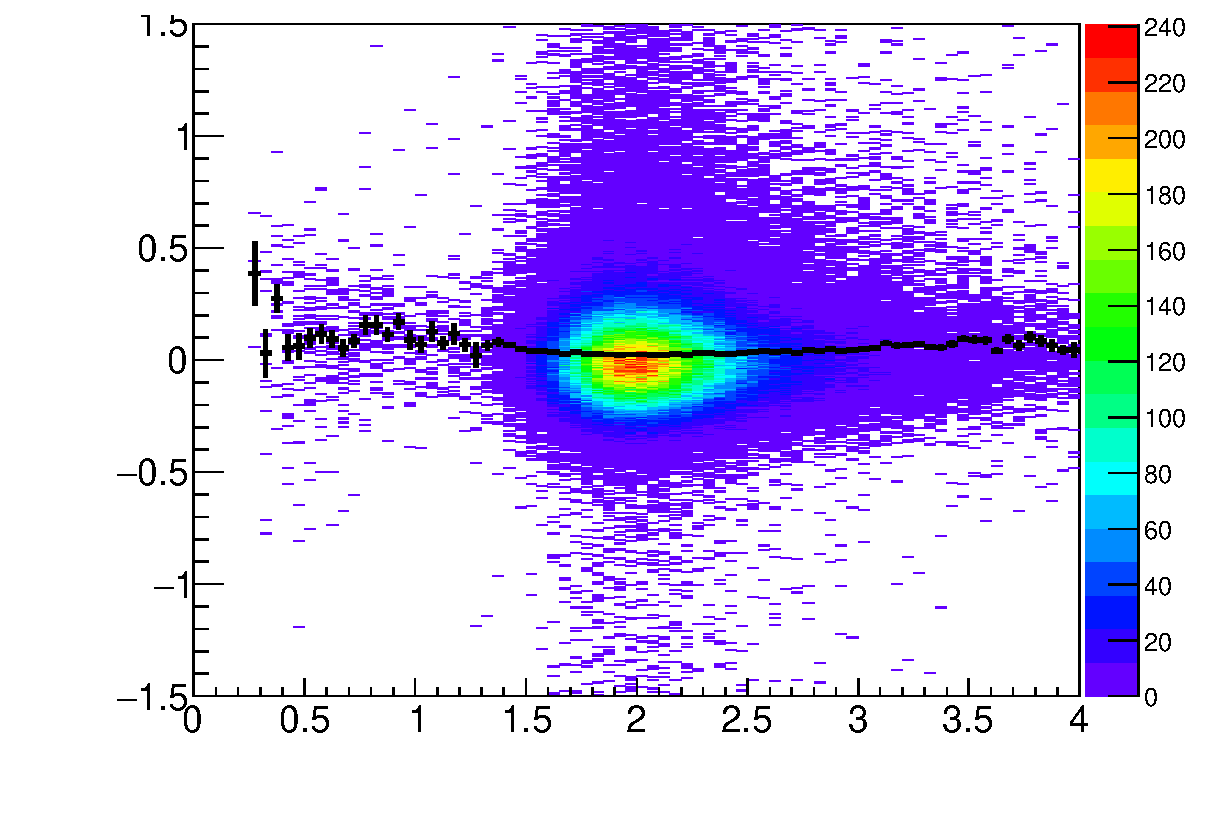
\includegraphics[width=5cm]{../pic/Dron/T0_slew_after.eps}
\end{minipage}
\end{tabular}
\caption{
  These figures indicate about slewing effect correction.
  These figures show the energy deposit of the T0 as the horizontal axis and the calculated time shift of T0-NC by the γ-ray as the vertical axis.
  The left figure shows about before correction, and the right figure shows about after correction. 
}
\label{fig:Slew}
\end{figure}

Hodoscope signals were read out as ADC and TDC data and chambers were read out only TDC. 
TDC data was converted to time.
The parameters for this were calibrated using time calibrator.
That module outputs two signals with a time difference of a certain constant multiple of time.

Hodscope had a correlation between ADC and time as shown in the left of Figure.\ref{fig:Slew} due to the rising edge of the signal.
The correlation was corrected as shown on the right of Figure.\ref{fig:Slew} by the follow function.

\begin{equation*}
  t_{corrected}=p_0+p_1 \frac{t}{\sqrt{dE}}+p_2 t
\end{equation*}

This collection was performed using a well-known timing signal.
For example, the Fig\ref{fig:Slew} shows the correction of the T0 using the $\gamma$--ray peak of the T0-NC TOF which has constant velocity.
This peak is also shown in Fig\ref{fig:NC_offset}.

Timing data of drift chambers was used to convert to the drift length.
The above figure of Fig\ref{fig:BLDC} shows the drift time distribution of the drift chamber installed at the beamline.
The middle figure indicates differentiated distribution which was used to decision start timing of each channel.
The bottom figure indicates integrated distribution which corresponds to conversion map from the drift time and the drift length by assumption that beam was uniformly irradiated on.

\begin{figure}[htbp]
\centering
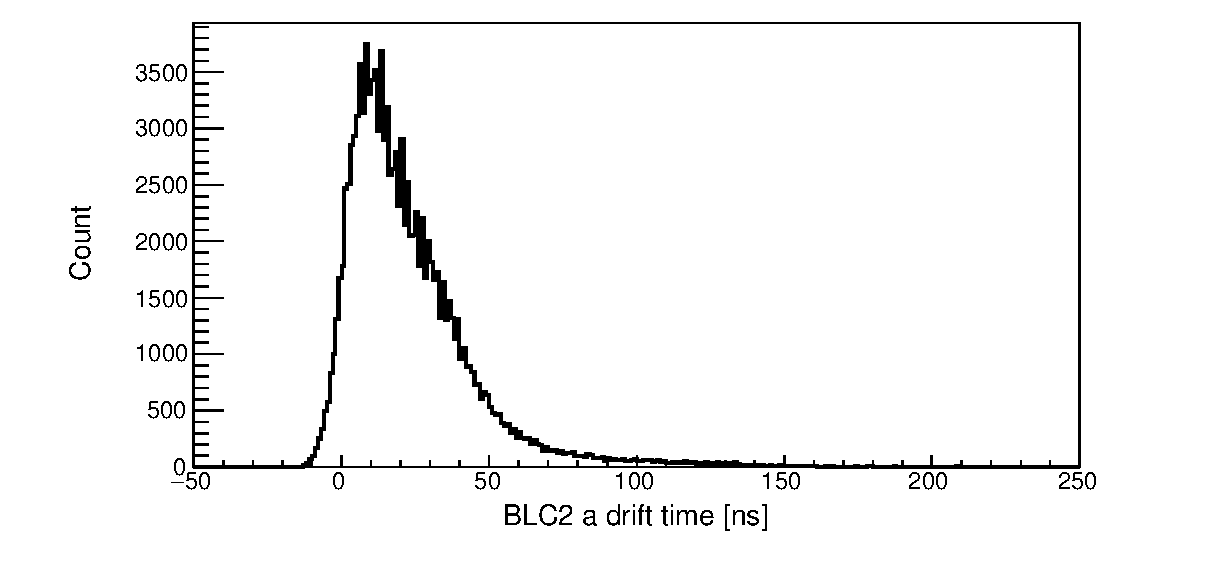
\includegraphics[width=10cm]{../pic/Dron/BLC2a_dt.eps}
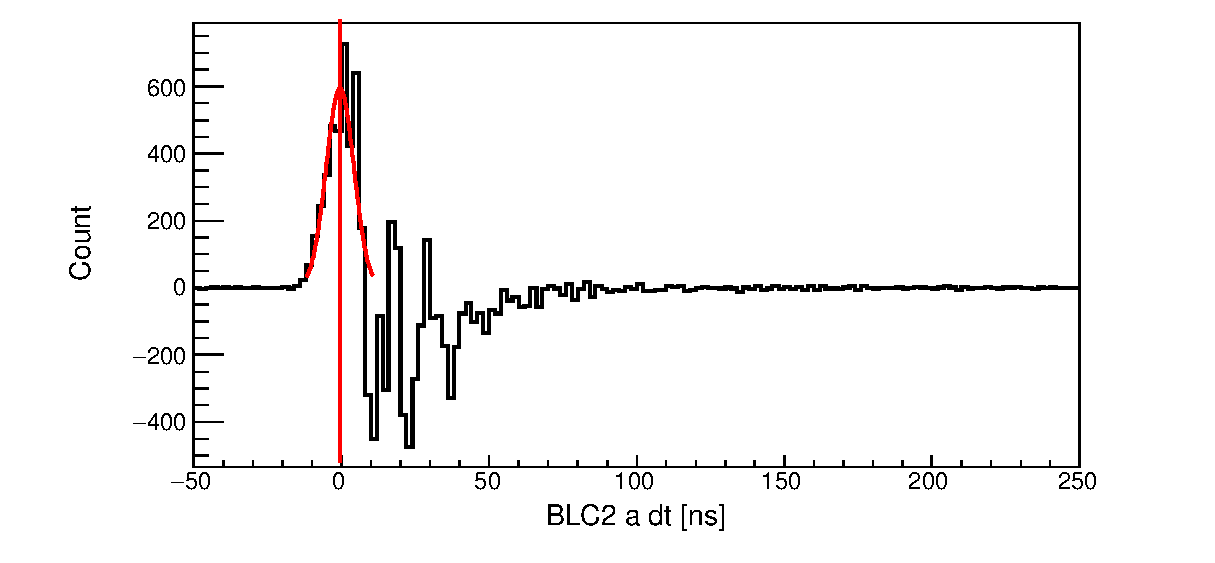
\includegraphics[width=10cm]{../pic/Dron/BLC2a_diff.eps}
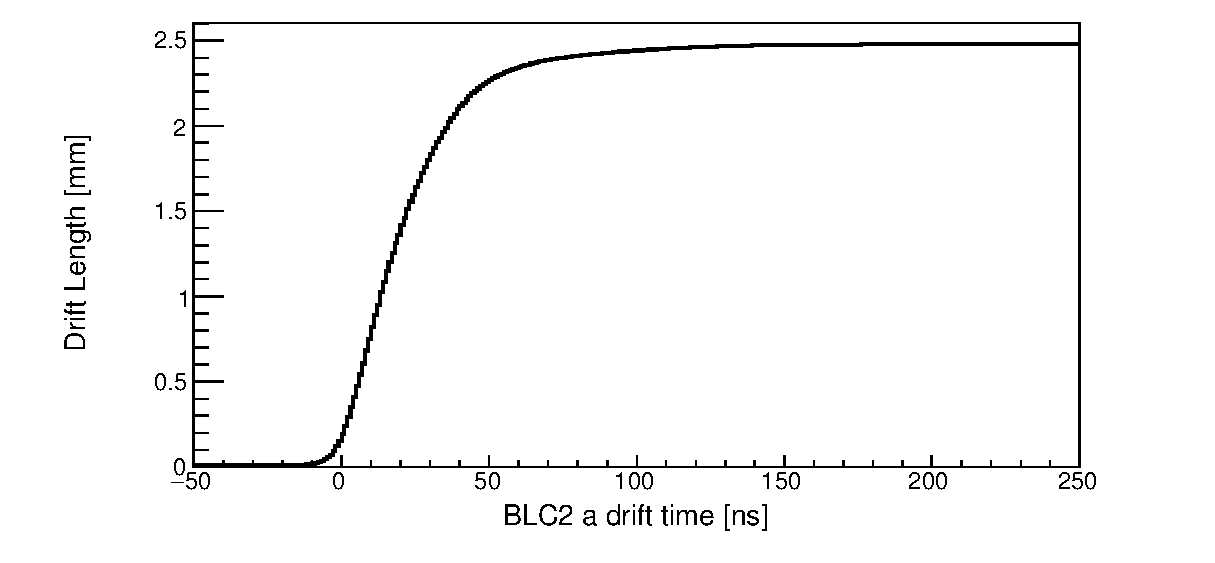
\includegraphics[width=10cm]{../pic/Dron/BLC2a_int.eps}
\caption{
  These figures indicate the calibration of drift chambers.
  The above figure shows raw distribution.
  The middle figure shows the start timing decision which is indicated by red lines.
  The bottom figure shows the $x$-$t$ map.
}
\label{fig:BLDC}
\end{figure}    
